\documentclass[11pt, letterpaper]{memoir}
\usepackage{HomeworkStyle}
\geometry{margin=1in}



\begin{document}

	\begin{center}
		{\large Quiz 17.1 -- Rate Laws}
	\end{center}
	{\large Name: \rule[-1mm]{4in}{.1pt} 


\subsection*{Initial Rate Method}
Consider the reaction: ~~ \ch{A + 2 B -> 3 C}. \\Below are graphs of the concentration of \ch{C} over time under three different initial conditions:

\noindent \hspace{-2em} 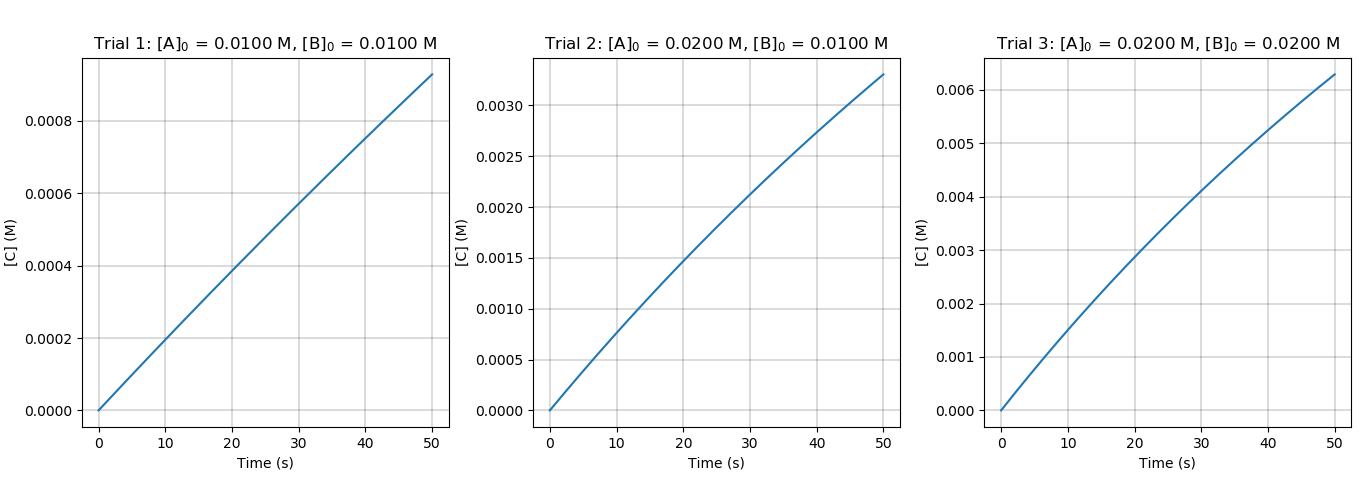
\includegraphics[width=1.1\linewidth]{Initial_Rates} 


\noindent $\circ$ From the data in the graphs, estimate the average reaction rate over the first $20~s$ for each trial

\vspace{8em}
\noindent $\circ$ Find the reaction order for both of the reactants, and the overall reaction order

\vspace{8em}
\noindent $\circ$ Give the value for the rate constant $k$, with appropriate units

\newpage
\subsection*{Half-Lives}
Radioactive decay follows \nth{1}-order kinetics \\Give the rate constant or half-life of the following radioactive elements

\begin{tabular}{c|c|c}
	Element & Half-life & Rate Constant $\left(\dfrac{1}{s}\right)$\\ \midrule
	\ch{^{14}C} & $5730~y$ & \hspace{6em} \\ \midrule
	\ch{^{57}Co} & \hspace{6em} & $2.95\times10^{-8}$ \\ \midrule
	\ch{^{99}Tc} & $6.0~h$ & \hspace{6em} \\ \midrule
	\ch{^{218}Po} & \hspace{6em} & $0.00373$ \\ \midrule
	\ch{^{3}H} & $12.3~y$ & \hspace{6em}
\end{tabular}

\noindent $\circ$ For each order of reaction, will the half-life increase, decrease, or stay constant over the course of a reaction?

\vspace{6em}
\subsection*{Integrated Rate Laws Method}
This quiz comes with a spreadsheet of data for three trials of the reaction:

\ch{A + B -> C}

\noindent Use the spreadsheet data to determine the complete rate law, including the rate constant with proper units and the reaction order with respect to each reactant


\newpage
\pagestyle{empty}
\addtocounter{page}{-1}	
\newgeometry{hmargin=0.9in,vmargin=1.25in}
\section*{\emph{O Me! O Life!}}
\paragraph{By Walt Whitman}~
\begin{verse}
	Oh me! Oh life! of the questions of these recurring,\\
	Of the endless trains of the faithless, of cities fill’d with the foolish,\\
	Of myself forever reproaching myself, (for who more foolish than I, and who more faithless?)\\
	Of eyes that vainly crave the light, of the objects mean, of the struggle ever renew’d,\\
	Of the poor results of all, of the plodding and sordid crowds I see around me,\\
	Of the empty and useless years of the rest, with the rest me intertwined,\\
	The question, O me! so sad, recurring—What good amid these, O me, O life?
	
	\hspace{9.5em}Answer.\\
	That you are here—that life exists and identity,\\
	That the powerful play goes on, and you may contribute a verse.
\end{verse}

\end{document}
